\documentclass[12pt]{article}
\usepackage[a4paper, margin=3cm]{geometry}
\usepackage{graphicx} 
\usepackage{csquotes}
\usepackage{booktabs}
\usepackage{soul} % for strikethrough \st{} and highlight \hl{}
\usepackage[dvipsnames]{xcolor} % Color names
\usepackage{hyperref}
\hypersetup{
    colorlinks=true,
    linkcolor=OliveGreen,
    anchorcolor=black,
    citecolor=OliveGreen,
    filecolor=black,
    menucolor=black,
    runcolor=black,
    urlcolor=OliveGreen}
\hypersetup{breaklinks=true}
\usepackage{url}
\usepackage{authblk}
\usepackage[final]{microtype}



% Bibliography information processing
\usepackage[
    backend=biber,
    style=apa,
    autocite=inline,
    sorting=nyt,
    sortcites=true,
    backref=false,
    backrefstyle=three,
    abbreviate=true,
    block=space,
]{biblatex}
% \DefineBibliographyStrings{american}{
%     backrefpage={Cited on p.},
%     backrefpages={Cited on pp.}
% }
\apptocmd{\sloppy}{\hbadness 10000\relax}{}{}
\appto{\bibsetup}{\sloppy}
\DeclareFieldFormat{apacase}{#1} % Title casing in APA
% \AtBeginBibliography{\small} % Can make the font in bibliography smaller

\addbibresource{../static/bibliography/parti.bib} %



% Languages, scripts, and fonts

% Font packages
\usepackage{libertine} % Latin, Greek, Cyrillic, Hebrew

% Fontspec
\usepackage{fontspec}
\defaultfontfeatures{Ligatures={TeX}}

% % Language settings
\usepackage[main=english, bidi=basic]{babel}

% Automatic typesetting of certain writing systems
\babelprovide[import=ar, onchar=ids fonts]{arabic}
% \babelprovide[import=he, onchar=ids fonts]{hebrew}
\babelprovide[import=sa-Deva, onchar=ids fonts]{sanskrit-devanagari}

% Define fonts (https://tug.org/FontCatalogue/)
% \babelfont{rm}{Linux Libertine}
% \babelfont{sf}{Linux Biolinum}
% \babelfont{tt}{Inconsolata}

\babelfont[*arabic]{rm}{Noto Naskh Arabic} % Amiri
% \babelfont[*hebrew]{rm}{Linux Libertine} % Noto Serif Hebrew
\babelfont[*devanagari]{rm}[Renderer=Harfbuzz]{Noto Serif Devanagari} 
% % Settigs: Scale=MatchUppercase; Scale=MatchLowercase; Scale=1.0; Language=Default

% East Asian scripts
% \usepackage{kotex} % Support for KR, JP, some TC (not SC).
% \setmainhangulfont{Noto Serif CJK KR} % Only on Overleaf
% \setmainhangulfont[
    % Path=./fonts/,
    % Extension = .otf,
    % UprightFont=*-Medium,
    % BoldFont=*-Bold
    % ]{NotoSerifKR}

\newfontfamily{\traditionalchinesefont}[
    Path=./fonts/,
    Extension = .otf,
    UprightFont=*-Medium,
    BoldFont=*-Bold
    ]{NotoSerifTC}

% \newfontfamily{\simplifiedchinesefont}[
%     Path=./fonts/,
%     Extension = .otf,
%     UprightFont=*-Medium,
%     BoldFont=*-Bold,
%     ]{NotoSerifSC}

% Other scripts
\newfontfamily{\tibetanfont}[Script=Tibetan]{Noto Serif Tibetan}

% Commands to use scripts
\newcommand{\bo}[1]{\tibetanfont{#1}\rmfamily}
\newcommand{\tc}[1]{\traditionalchinesefont{#1}\rmfamily}
\newcommand{\zh}[1]{\simplifiedchinesefont{#1}\rmfamily}

% Keywords command
\providecommand{\keywords}[1]{\small\noindent\textbf{\textit{Keywords ---}}#1}

% ORCiD
\definecolor{orcid}{HTML}{A6CE39}
\usepackage{academicons}
\newcommand{\orcid}[1]{\href{https://orcid.org/#1}{\textcolor{orcid}{\aiOrcid}}}



\title{A new etymology for Chinese \tc{豆蔻} \textit{dòukòu} `cardamom; nutmeg' }
\author[1]{{\small\orcid{0000-0003-2042-4655}}~Gábor Parti}
\author[2]{{\small\orcid{}}~Ian Joo}
\affil[1,2]{The Hong Kong Polytechnic University}
\affil[2]{Nagoya University of Commerce and Business}
\date{\small{February 2024}}

\begin{document}

\maketitle

\begin{abstract}
    This paper offers a new etymological explanation for the Chinese word \tc{豆蔻} \textit{dòukòu} `cardamom; nutmeg' and explores the possibilities of its trade-language origins. We propose that this Chinese word is a loanword that could have arrived via Southern Min, from an Indian Ocean trade-language used on the ancient Maritime Silk Road during the Tang dynasty. We think this word have entered the Chinese lexicon together with the economic products it denotes, and went through phono-semantic matching. We introduce our reasoning in four main points, and detail out four sets of observations regarding 1) the first written records, 2) character composition, 3) available lexicographical data, and 4) a range of seemingly related regional \textit{Wanderwörter} (wandering loanwords) as evidence supporting our hypothesis. In uncovering this word's lexicogenesis, we also discuss the linguistic and historic plausibility of our claims, and  explore possible candidate etymons from relevant Indic and Austronesian languages.

    ---

    Cardamom is a popular spice with a history spanning thousands of years of culinary and medicinal use. In fact, cardamom can refer to multiple kinds of fragrant fruits, besides the well-known green seed-pods of “true cardamom”, Elettaria cardamomum. Moreover, if we dive deeper into the identities of cardamoms from an Asian perspective, we find a conundrum of words and materials. Prototypical cardamoms are botanically different species in various regions (e.g., Java, Indochina, Yunnan, India), and their names got confused along the paths of diffusion. In the present study, we look at the situation in Chinese, where the corresponding word is dòukòu \tc{豆蔻}, also pointing towards nutmeg (Donkin 2003). Dòukòu first appears as báidòukòu [white-cardamom] in a Tang-era miscellany called Youyang Zazu, where it is reported to come from the land of Kakkola, describing round cardamoms (Wurfbainia compacta) originally sourced from Siam or Java. According to this 9th-century source, the spice is called \tc{多骨} duōgǔ, and the perceived Middle Chinese pronunciation, /tɑ-kuət̚/, makes possible for it to be a transcription of an Indo-Aryan word, e.g., Pali takkola or Sanskrit kakkola. On the other hand, the same does not apply for \tc{豆蔻} dòukòu, whose Middle Chinese pronunciation would be /dəuH-həuH/. As an alternative, we propose that dòukòu could be a loan via Southern Min. Based on Kwok's reconstruction of Proto-Southern-Min, the equivalent of dòukòu would be /*tɑu-khɑu/ (Kwok 2018; B.-Ch. Kwok, personal communication, August 17, 2022), more similar to the Indic words. This is historically plausible, given that Fujian was in direct contact with the maritime traders responsible for the bulk of the spice trade, and that Sanskrit was one of the main languages of the Srivijaya Empire encompassing Kakkola around this time. In this brief etymological study, we clear the air around cardamom nomenclature, and reveal a possible trace that Fujianese traders have left on modern Chinese. This is not only interesting in terms of food history, but also in terms of the linguistic history of Chinese, as few loanwords from Southern Min have made their way into Middle Chinese.

\end{abstract}

\noindent{\small\textbf{\textit{Keywords --- }} Cardamom, \tc{豆蔻}, Etymology, Trade-language, Chinese, Southern Min, Indian Ocean, Spice Trade}

\section{Introduction}

\subsection{Cardamom conundrum}

Introduce what is cardamom a bit.

\subsection{What is cardamom?}

What do people mean under the name \textit{cardamom} depends on who we ask, where we are, and in what language we are operating in---for the word \textit{cardamom} and its translations can refer to multiple different spices. In all cases, this name will refer to an aromatic plant, yielding a culinary and medicinal spice, and in all likelihood, most readers will think of the dried fruits of \textit{Elettaria cardamomum} (L.) Maton, seen in Figure \ref{fig:cardamom}.

The botanic organization of cardamoms started with Linneaus, and it is still changing, Burkill lamented on misnaming some almost a hundred years ago \parencite{burkill_1930_cardamoms}.

\begin{figure}[!ht]
    \centering
    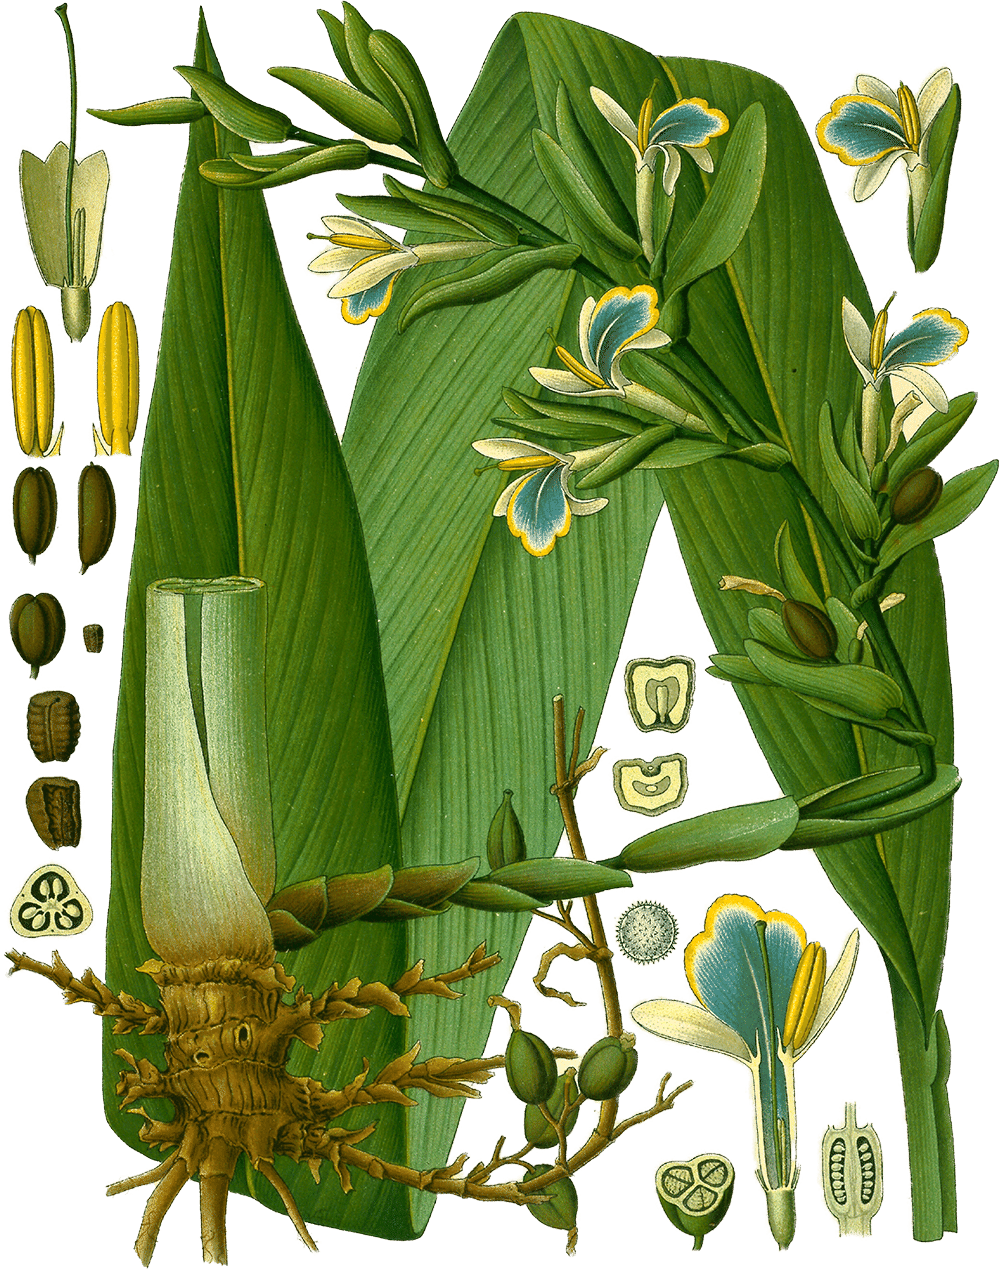
\includegraphics[width=0.45\textwidth]{../static/images/illustrations/cardamom.png}
    \caption{\textit{Elettaria cardamomum} in \tvolcite[]{2}[186]{koehler_1887_koehler}'s \textit{Medizinal Pflanzen}}
    \label{fig:cardamom}
\end{figure}

\textit{Elettaria cardamomum} (L.) Maton is an aromatic flowering plant from the ginger family (\textit{Zingiberaceae}), native to India's Western Ghats ??, the mountain range trailing above the Malabar coast of Kerala. This is the same region where black pepper hails from, and in an Indian context they are often called ``the king and queen of spices'' \parencite{nair_2020_geographya}. 

It is a well known culinary spice with a long history, also used in the infusion of beverages, and perfumery (e.g., Indian cuisine; Arabian coffee). It was used in India since the Vedic period ??, and it was traded to and through Mesopotamia since the bronze age \parencites{parry_1969_spices}{ravindran_2002_cardamom}. 

It was known in Europe since antiquity and used as medicine; Greek historians and physicians wrote about its healing properties, sometimes even correctly noting that it comes from India. Today it is still valuable, it is the 3rd most expensive spice after saffron and vanilla. It is also known as green cardamom and true cardamom.  


It is a well known culinary spice, also used in the infusion of beverages and perfumery (e.g., Indian cuisine; Arabian coffee), with a long history. It was used in India since the Vedic period, and it was traded to and through Mesopotamia since the bronze age. It was known in Europe since antiquity and used as medicine; Greek historians and physicians wrote about its healing properties, sometimes even correctly noting that it comes from India. Today it is still valuable, it is the 3rd most expensive spice after saffron and vanilla. It is also known as green cardamom and true cardamom.

native to India’s Western Ghats – so as black pepper; “the Queen of Spices”
Popular spice used in cooking and beverages, perfumery, (e.g., Indian cuisine, Arabian coffee), 
Used medicinally in India since Vedic times
Traded to Mesopotamia since the Bronze Age (Parry, 1969; Ravindran, 2002)
Known in Europe since Antiquity – Theophrastus, Dioscorides, Pliny (Anderson, 2023)
3rd most expensive spice today
a.k.a. green cardamom, “true cardamom”



In Europe, India, the Middle East, the name cardamom refers to the seed pods of Elettaria cardamomum, 
an aromatic flowering plant from the ginger family, 
native to India’s Western Ghats, above the coasts of Kerala. This is the same region where black pepper hails from, and in an Indian context they are often called “the king and queen of spices”.
It is a well known culinary spice, also used in the infusion of beverages and perfumery, with a long history. 
It was used in India since the Vedic period, and 
it was traded to and through Mesopotamia since the bronze age. 
It was known in Europe since antiquity and used as medicine; Greek historians and physicians wrote about its healing properties, sometimes even correctly noting that it comes from India.
Today it is still valuable, it is the 3rd most expensive spice after saffron and vanilla.
It is also known as green cardamom and true cardamom.

---

False cardamoms

The name true cardamom implies the existence of “false” ones.
Not so strange in spice nomenclature: alternative economic products; adulteration
Many other aromatic plants in the ginger family referred to as cardamoms
Native to Asia (Amomum genus) and Africa (Aframomum genus)
Why are these other spices called cardamoms as well?
Common feature: aromatic seed-pods containing small seeds.

What is considered “false” is determined by the reigning prototype spice in a given culture (whether native or first encountered), and the perceived value (cf. true cinnamon vs. bastard cinnamon).

Wait a minute, true cardamom? Are there false cardamoms? Well, yes! The name “true cardamom” implies the existence of “false” ones, at least in an English context.
This is not that strange when it comes to spice names and it hints on the availability of alternative products, or to practices of adulteration. 
In fact, there are at least a dozen other plants in the ginger family to which the botanical and culinary literature refer to as cardamoms, 
native to Asia and Africa in the genera Amomum and Aframomum.
So, why are these other spices called cardamoms as well? Because of their physical, chemical, and functional similarity, but especially one distinct feature: they are all aromatic seed-pods containing small seeds. 
By the way, no one in Asia thinks these cardamoms are fake, what is considered “false” is determined by the reigning prototype spice in the given culture (whether it grows there, or it’s the first of its kind they have encountered), and the perceived value of the spice (so called true cinnamon from Ceylon was and is considered superior to cassia or Chinese cinnamon, warranting names such as bastard cinnamon).

---

So, while for many of us cardamom looks like this,

---

Some other prototype cardamoms of Asia

There are places where the “default”, prototype cardamom looks and tastes a bit different.
In Northern India, Nepal, Bhutan, Bengal, there is black cardamom, or greater cardamom – you can see it on the left; in Yunnan, Southwestern China there is the even larger tsaoko cardamom, or Chinese black cardamom; and Thailand, Cambodia and Indonesia have two species that yield little round white cardamoms. 

---

Some common names in English

amomum, bastard cardamom, bastard Siamese cardamom, Bengal cardamom, big cardamom, black cardamom, brown cardamom, Cameroon cardamom, Chinese black cardamom, Chinese cardamom, Ethiopian cardamom, fake cardamom, false cardamom, greater cardamom, green cardamom, Guinea cardamom, hill cardamon, Indian black cardamom, Indian cardamom, Indonesian cardamom, Java cardamom, Java round cardamom, Java white cardamom, kepulaga, korarima, krervanh, large cardamom, Madagascar cardamom, Malabar cardamom, Nepal cardamom, round cardamom, round Chinese cardamom, Siam cardamom, Tavoy cardamom, Thai cardamom, true cardamom, tsao-ko cardamom, wild Siamese cardamom, winged cardamom, Yunnan cardamom…

Selected sources: Dalby (2000); Prance \& Nesbitt (2005); van Wyk (2014); Hill (2017); Anderson (2023), etc.  



All of these have a bunch of other vernacular names in English, usually named after the green cardamom as the prototype spice, modified with an adjective of color, a place of origin, or both; occasionally using a native name.

I have collected these names from the botanical literature, books on the history of spices and so on. You don’t have to read these, I just wanted to show you how cardamom is used as a prototype word in the generation of names for novel spices.

---

All the relevant spice bearing plants…

Alpinia galanga (L.) Willd. 
Alpinia globose (Lour.) Horan. syn. Amomum globosum Lour.
Alpinia hainanensis K.Schum. syn. Alpinia katsumadai Hayata
Amomum maximum Roxb.	
Amomum subulatum Roxb.	
Elettaria cardamomum (L.) Maton syn. Amomum cardamomum L.
Hornstedtia costata (Roxb.) K.Schum. syn. Amomum costatum (Roxb.) Benth. ex Baker
Lanxangia tsao-ko (Crevost \& Lemarié) M.F.Newman \& Skornick. syn. Amomum hongtsaoko Liang et Fang; A. tsao-ko Crevost et Lemaire
Wurfbainia aromatica (Roxb.) Škorničk. \& A.D.Poulsen syn. Amomum aromaticum Roxb.
Wurfbainia compacta (Sol. ex Maton) Škorničk. \& A.D.Poulsen syn. Amomum compactum Sol. ex Maton; Amomum kepulaga Sprague \& Burkill
Wurfbainia vera (Blackw.) Škorničk. \& A.D.Poulsen syn. Amomum krervanh Pierre \& Gagnep.; Amomum kravanh Pierre ex Gagnep.
Wurfbainia villosa (Lour.) Škorničk. \& A.D.Poulsen syn. Amomum villosum Lour.
Aframomum melegueta K.Schum.	Aframomum grana-paradisi (L.) K.Schum. 
Aframomum cereum (Hook.f.) K.Schum. syn.Aframomum sceptrum (Oliv. \& D.Hanb.) K.Schum.
Aframomum exscapum (Sims) Hepper	
Aframomum alboviolaceum (Ridl.) K.Schum. syn. Aframomum macrospermum (Sm.) Burkill
Aframomum angustifolium (Sonn.) K.Schum.	
Aframomum corrorima (A.Braun) P.C.M.Jansen	 syn. Amomum korarima J.Pereira
Aframomum daniellii	(Hook.f.) K.Schum. syn. Aframomum hanburyi K.Schum.

Now, the whole range of plants from the cardamom-group is long and unnecessary, but now we have a question: Which one is doukou?

---

Well, the answer is: a few of these, and more. In a Chinese context we have our not so well-known green cardamom, black cardamom from the Himalayas, the two white cardamoms from Southeast Asia, some semi-exotic ones that look like tiny brains, and the reddish fruits of galangal.

Alpinia galanga (L.) Willd. 
Alpinia hainanensis K.Schum.	
Amomum subulatum Roxb.	
Elettaria cardamomum (L.) Maton 
Wurfbainia compacta (Sol. ex Maton) Škorničk. \& A.D.Poulsen
Wurfbainia vera (Blackw.) Škorničk. \& A.D.Poulsen

---

X cardamom  = X豆蔻 x dòukòu



Here is a table showing the same plant products with their Chinese names; consider the examples: red-cardamom, fragrant-cardamom, little-cardamom, white-cardamom, and so on.
You can see that Chinese doukou corresponds to cardamom; at least on a pragmatic level if not botanically. 
Dòukòu is a generic term and Chinese too also adds additional modifiers of color, place, or some other feature, with many-many dialectal variations that are out of scope for now, but basically we have a formula.
As bonus, we also have nutmeg, which is called ròudòukòu (flesh cardamom) in Chinese.

---

Nutmeg

It is a seed of a tree of an unrelated species from a different family, native to the Maluku islands of Indonesia, famously called the Spice Islands in colonial times, and until the 18th century it only grew here. It was one of the most prized products of the spice trade, for half a kilo you could buy a house in London. 


---

Origins

Map

South \& Southeast Asia
Biodiversity hotspot
Maritime Silk Road

By the way, these aromatic plants come from this region surrounding Mainland Southeast Asia, which is a biodiversity superhotspot, with many stops along the Maritime Silk Road.









\section{Etymological breadcrumbs}

Scholars have a realively good understanding of the etymology of the English word \textit{cardamom}, which is usually reconstructed along the following lines:

\begin{quote}
    \textbf{English} \textit{cardamom} `cardamom' ca. 1425, via \textbf{post-classical Latin} \textit{cardimomum}, a. 1398
    < later also from \textbf{Old French} \textit{cardemome} `cardamom', ca. 1170; cf. modern French \textit{cardamome}
    < \textbf{Latin} \textit{cardamōmum} `cardamom', 1st c. AD
    < \textbf{Hellenistic Greek} {καρδάμωμον} \textit{kardámōmon} `cardamom', haplological κάρδαμ- \textit{kárdam-} `cress' + ἄμωμον \textit{ámōmon} `an Indian spice plant', 3rd c. BC
    < \textbf{Ancient Greek} {κάρδαμον} \textit{kárdamon} `garden cress, \textit{Lepidium sativum}', prehaps a loanword (many plant names with \textit{-amon} are clear loanwords; the suffIx \textit{-amon} is known from Pre-Greek), ultimately of uncertain origin, 4th c. BC; cf. cognates classical Latin \textit{cardamum}
    \parencites[s.v. cardamom]{oed}[s.v. cardamome]{tlfi}[s.v. cardamomum]{lewis_1879_latin}[s.v. καρδάμωμον]{liddell_1940_greekenglish}[s.v. κάρδαμον]{liddell_1940_greekenglish}[644]{beekes_2010_etymological}
\end{quote}

Kárdamon was identified with the word 𐀏𐀅𐀖𐀊 ka-da-mi-ja 41 , (kardamia as a feminine form of kardamon) appearing on Mycenaean tablets listing spices in Linear B, excavated in the “House of the Sphinxes” in 1950s, and dated to the 1200s bc (Bennett et al., 1958, p. 107).



this is how linguists usually reconstruct word histories: tracing word stages step by step. Basically cardamom came via Old French and Latin from a Greek word. I said kinda, because the exact origins are uncertain. And may or may not appear on Mycenaean stone tablets written in Linear B over 3000 years ago, it is outside of my specialty to judge these claims. It is quite difficult to be sure about the source of a word at this time-depth, almost 3000 years ago.

What about the etymology of doukou? Well, we had some suspicions, and during our investigations we came across various pieces of evidence that led us believe that doukou is a loanword. I will now introduce our observations and reasons why we think so in 4 points.

\subsection{First mentions, first confusions}

The first recorded mention of \tc{豆蔻} \textit{dòukòu} is from a 9th-century book called \tc{酉陽雜俎} \textit{Youyang Zazu} [\textit{Miscellaneous Morsels from Youyang}], which is a Tang era miscellany of tall tales and legends, strange phenomena, fantastic creatures, and exotic products -- but also an excellent source of historical data. It was collated by Duan Chengsi (d. 863), and in \hl{``chapter'' (juan (scroll, or book))} 18 he discusses 24 foreign plants, which have been imported to China or have been brought as tribute from faraway places, such as Magadha (in India), Malaysia, Persia, Silla (Korea), and Syria, often reporting the local names for the non-native plants and products, and usually compares them to something more familiar to his readership. We can find descriptions of acacia, Balm of Giliad, galbanum, jackfruit, jasmine, and Narcissus, among others \parencite{reed_2003_tang}. Section 55 tells us about cardamom, the text is accessible via the Chinese Text Project\footnote{\url{https://ctext.org/wiki.pl?if=en&chapter=801324}} \parencite{sturgeon_2021_chinese}, the translation is from us.



\begin{quote}
    \tc{\textbf{白豆蔻},出\textcolor{OliveGreen}{伽古羅}國,呼為\textcolor{OliveGreen}{多骨}。\\
    形如芭焦,葉似杜若,長八九尺,冬夏不凋。\\
    花淺黃色,子作朵如蒲萄。其子初出微青,熟則變白,七月採。}
    
    \textbf{White cardamom}, comes from the country of \textcolor{OliveGreen}{Kakula}, called \textcolor{OliveGreen}{/tɑ-kuət̚/}. [\dots]

    \begin{flushright}
        \addvspace{-2ex}
        (YYZZ §18:55)
    \end{flushright} 
\end{quote}

After stating the place of origin and its name, the author then proceeds to describe the plant's morphology: its height, its leaves, its yellow flowers, compares the shape of the fruits to grapes (also a \hl{foreign} plant in China), and puts the time of harvest to the seventh month of the lunar calendar.

\hl{...Middle Chinese reconstructions}

The fist obvious question here is: Why is it ``white'' cardamom? Or to put it more precisely, why does cardamom already have a modifier when it is the first attested instance we have of this word? According to \textcite[22]{donkin_2003_east}, the Chinese first confused nutmeg and cardamom, ``doubtless on account of a resemblance between their fruits''. We also know, that in the earliest sources, both spices were referred to as \textit{dòukòu} \parencites{hsu_1967_notes}{donkin_2003_east}, and that both were sourced from mainland Southeast Asia, and carried up to the Tang courts on ships from Kakola \parencite[184-185]{schafer_1985_golden}. This place also appears in Ibn Battuta \parencite{dunn_1986_adventures}


To avoid nomenclatural confusion, nutmeg became 肉豆蔻 ròudòukòu, cardamom became 白豆蔻 báidòukòu.
This mix-up exists in other languages as well!

According to Donkin, the Chinese first confused nutmeg with cardamom, on account of their similar fruits, and at some point both imported spices were called doukou.
Furthermore, both were sourced from mainland Southeast Asia, likely traded on the same trade routes, and the same ships, ((He says that, nutmeg was known in Chinese as kakola (ca. 725), and later as doukou (ca. 863), roudoukou is the name in later sources, including an illustrated herbal of 1062 (1249).))
So, to avoid confusion nutmeg became roudoukou – flesh cardamom – while the round cardamoms became baidoukou – white cardamom.
As many scholars noticed before, the confusion is not limited to Chinese.

((Nutmeg: “chia-kou-le” (ca. 725), as “to-ku” (ca. 863). “jou-tou-k’ou” (ca. 1062)
White cardamom: “tou-k’ou”, “pai-tou-k’ou” (Hsü, 1967; Donkin, 2003)))



\subsection{Character characteristics}

Our word under scrutiny is made up of two characters, \tc{豆} \textit{dòu} and \tc{蔻} \textit{kòu}. \textit{Dòu} is relatively straightforward, in dictionaries you can find definitions, such as `bean'; `pod-bearing plant or its seeds'; `bean-shaped object'; etc. ?? \textit{Kòu} on the other hand is much more specific, and dictionary entries usually direct the reader to other entries where the character is used, e.g., `used in 豆蔻'; `see豆蔻 nutmeg, cardamom'; etc. ?? The case in point here is that \textit{kòu} does not mean anything else, and it does not appear in other word, which is rare for a Chinese character. 

\tc{蔻} \textit{kòu} is made up of the radical for grass, \tc{艹} \textit{cǎo} `grass, herb' ??, and a phonetic component \tc{寇} \textit{kòu} meaning `bandit' which is a typical phono-semantic compound in Chinese. This sinogram however does not seem to exist before its emergence in the word for the spices, there is no record of \tc{蔻} \textit{kòu} before the 9th century. Was this character created for this purpose? It seems so. And if yes, then where does the \hl{/kou/ sound} come from? We think it is likely a loanword.

Furthermore, doukou often appears in a form ?? where the first character too has the grass radical on top (i.e., \tc{荳蔻}). Featuring the grass radical on both characters seems to be a typical device in the naming foreign edible plants, often loanwords themselves. Cf. the Chinese words \tc{草莓} \textit{cǎoméi} `strawberry', \tc{菠菜} \textit{bōcài} `spinach', and an archaic\footnote{The modern word for cumin, \tc{孜然} \textit{zī​rán} comes via Uyghur, \hl{from Sanskrit?}} word for `cumin', \tc{蒔蘿} \textit{shíluó} `cumin'.

\subsection{Lexicographical clues}

Youwei Shi (2021) Loanwords in the Chinese Language. Routledge:
	“Doukou 豆蔻, meaning cardamom, introduced to China in the 	Tang dynasty, probably originated from Arabic takur, related to 	the name of the ancient port Takola.” (p. 44)
No Arabic word like takur
Points to a place: Takola.

---

So, I tried to check what the dictionary says. Chinese is one the few major languages with no authoritative etymological dictionary, but there are some works on loanwords in Chinese. The most recent publication on this topic has an entry on doukou, and it says: 
…
This sounds like an crucial claim to push our investigation forward, 
but sadly, Arabic does not have a word that sounds or looks like takur
it does on the other hand point to an ancient port: Takola, which sounds awfully familiar to Kakola.





\subsection{The sea of kakkola/takkola type words}

Arabic قاقلة qāqulla ‘cardamom’ < Aramaic < Akkadian < Sanskrit?
Sanskrit कक्कोल kakkola ‘species of plant (bearing a berry, the inner part of which is waxy and aromatic’/ तक्कोल takkola *‘Pimenta acris’ (Monier-Williams, 1899, pp. 241, 431)
Pali takkola ‘perfume made from an aromatic berry’ (Pali Text Society, 1921–1925, p. 292),
Tibetan ཀ་ཀོ་ལ kakola ‘black cardamom’ (Amomum tsao-ko) (Goldstein et al., 2001, p. 1), 嘎哥拉 gágēlā in Eastern Tibet (Hu, 2005)
Javanese ꦏꦥꦸꦭꦒ kapulaga?, Malay pelaga? …etc.
Kakola (Chinese: Kakula, Arabic: Qāqulla) was a trading emporion on the western coast of Malay peninsula known in Ancient Greece as Takola of the golden Chersonese in Ptolemy’s Geography, AD 2nd c., and Talaitakkōlam in Tamil based on inscriptions from Chōla expeditions, AD 10th c. (Wheatley, 1961, p. 270).

---

There is an Arabic word for cardamom, qāqulla, which is not a native word. It is usually traced back to Sanskrit via Aramaic and Akkadian.
Looking up the Sanskrit word will send us down a rabbit hole about kakkola/takkola, a word that is the proposed etymon for others, such as Pali takkola, Tibetan kakola, and many more, including Javanese and Malay.
Kakola has been identified as Takola, an old trading emporion on the western coast of the Malay peninsula, already known to Ancient Greek geographers like Ptolemy, and also recorded in Tamil inscriptions of Chola expeditions.
The 4th reason therefore is about a regional review of seemingly related words, the technical word for these are Wanderwort of Kulturwort using German. 


(Just as the use of cinnamon may have led to the discovery of cloves, so one or other of the many cardamoms grown in South China and mainland South East Asia probably predisposed the Chinese to the imported nutmeg Takkola (Chinese Ko-ku-lo, Arabic) was a place or region on the west coast of Malaya,170 which the Chinese from the eighth century thought produced both nutmegs and the round cardamom (Amomum kepulaga), the latter possibly introduced from Java.171)



Other people have already noticed this before. Here is a collection of all the takkola/kakkola type words around the Indian Ocean world; the words usually have the sense of some aromatic substance or spice. 
Historians place the ancient port of Takola here, marked with the red dot, and we know from Chinese sources that the Chinese have imported products from here, so
Now the question is: Could 豆蔻 dòukòu be an eponymous loan related to one of these names? Could this transmission happen?






\printbibliography

\end{document}
